\documentclass{article}
\pdfpagewidth=8.5in
\pdfpageheight=11in
\usepackage{ijcai27}
\usepackage{times,url}
\usepackage[hidelinks]{hyperref}
\usepackage[utf8]{inputenc}
\usepackage[small]{caption}
\usepackage{microtype,amsmath,amssymb,amsthm,booktabs,graphicx,array}
\usepackage[switch]{lineno}
\linenumbers
\urlstyle{same}
\newcommand{\citep}{\cite}
\pdfinfo{/TemplateVersion (IJCAI.2027.0)}
\newtheorem{theorem}{Theorem}
\newtheorem{proposition}[theorem]{Proposition}
\newtheorem{corollary}[theorem]{Corollary}
\newcommand{\E}{\mathbb E}
\newcommand{\KL}{D_{\mathrm{KL}}}
\newcommand{\TV}{\operatorname{TV}}
\newcommand{\Var}{\operatorname{Var}}
\newcommand{\sig}{\operatorname{sigmoid}}
\title{CAEA: Auditing and Repairing Preference-Induced Belief Feedback}
\author{}
\begin{document}
\maketitle


\begin{abstract}
Pooled single-turn evaluations can miss whether an assistant amplifies
belief differences over repeated interactions.
We demonstrate this gap in a controlled binary response model: increasing
agreement pressure leaves the entire pooled response--outcome distribution
unchanged, while the mean-response dynamics change from convergence to
separated stable beliefs. We study conflict-aware epistemic alignment
(CAEA), which repairs an externally audited content distribution while
retaining the preference policy within each content class. Classical KL
projection quantifies the preference cost; coupling bounds relate repair
strength to feedback contraction. Finite stance audits cannot certify
global stability without additional regularity; a known curvature bound
yields a finite-sample certificate. An extension preserves this ambiguity at arbitrarily small report regret. Ten-seed finite-action DPO experiments,
stochastic simulations, and two frozen-language-model candidate-selector
pilots illustrate these results and their limits. Full repair and audit-only
have identical forecast risk by construction. Soft-score reweighting can
achieve a better risk--KL tradeoff, and option permutations remove the
pilots' initial DPO gains. The contribution is an analysis of audit
observability, conditional repair, and stability under explicit assumptions;
it does not establish benefits for human cognition or free-text generation.
\end{abstract}


\section{Introduction}
Preference judgments can reward agreement over truthfulness \citep{sharma2024},
but agreement can also be warranted. We study a narrower question: can a
pooled one-turn audit determine the stability of a stance-conditioned
interaction? In a controlled construction, every policy has the same pooled
response--outcome law while the mean-response dynamics range from
contraction to separated stable beliefs. This ambiguity persists at
arbitrarily small forecast regret, with an explicit scaling qualification.

Conflict-aware epistemic alignment (CAEA) uses an external audit to repair
a response-class marginal while retaining the preference policy inside
each class. The projection is classical. Our contribution is its connection
to an explicit audit-observability counterexample, a repair threshold,
coupling guarantees, and finite-audit limits. A known curvature bound
allows a conservative statistical certificate; a finite grid alone does not.

The empirical contribution is controlled verification and failure analysis.
Shared target information explains the identical report risks of full
repair and audit-only; intermediate risk and target-TV changes follow
algebraically. Conditional preference retention can fail to preserve
aggregate style, and the frozen-neural pilot fails an option-permutation
control. We do not claim a new general projection principle, robust
free-text post-training, or validated benefits for human belief formation.

\section{Related work}
\paragraph{Preference optimization and agreement.}
DPO uses policy/reference likelihood ratios \citep{rafailov2023}; sycophancy
has empirical connections to preference judgments \citep{sharma2024}.
Shapira et al.\ derive a closest-KL anti-amplification correction
\citep{shapira2026}, the direct antecedent to our projection component.
Moya et al.\ study spurious learning and tie training \citep{moya2026}.
We focus on what pooled and finite stance audits can certify about feedback.

\paragraph{Updating and dynamics.}
BASIL separates sycophantic shifts from rational updating \citep{atwell2026};
Ma et al.\ show the need to preserve informative updating \citep{ma2026}.
PlurPO uses multiple stakeholder perspectives \citep{hatgis2026}.
Ghosh et al.\ already study nonlinear sycophantic belief dynamics and
attractors \citep{ghosh2026}; multiple stable beliefs alone are not our
novelty claim. Our construction explicitly equates pooled audit laws
across different feedback regimes and accounts for repair strength.

\paragraph{Classical ingredients.}
The repair follows from information projection \citep{csiszar1975};
proper-score regret follows scoring-rule theory \citep{gneiting2007}.
Contraction arguments for random iterations are classical
\citep{diaconis1999}. Diversity optimization \citep{lanchantin2025} addresses
a different objective from matching a justified report target.

\section{Problem formulation}
Let $x$ denote shared admissible evidence and $s\in[0,1]$ a user's stated
probability. Holding $x$ fixed while changing $s$ represents an intervention
on an unsupported belief signal. Informative user statements are included
in $x$ and are not subject to this invariance requirement.

The response space $\mathcal Y$ is finite. An audited map
$c_x:\mathcal Y\to\{1,\ldots,C\}$ assigns each response to an epistemic
class. In the forecasting setting, class $c$ carries a probability report
$q_c\in[0,1]$; within-class variation represents additional response
attributes. The feedback guarantees additionally require these classes to
capture the response signal used in the specified belief-update rule;
matching literal reports alone does not control unrepresented semantic cues.
Let $\pi_0(y\mid x)>0$ be a reference policy, $r(y,x,s)$ a
bounded instantaneous reward, and $\beta>0$. Define
\begin{equation}
 \begin{aligned} J_{x,s}(\pi)&=\E_\pi r(Y,x,s)-\beta\KL(\pi\|\pi_0),\\
 \pi_P(y\mid x,s)&=\frac{\pi_0(y\mid x)e^{r(y,x,s)/\beta}}{Z_{x,s}}.\end{aligned}
 \label{eq:gibbs}
\end{equation}
The Gibbs policy $\pi_P$ is the ideal distributional maximizer. Relating
it to finite-sample DPO requires a compatible preference model, support,
and sufficient policy expressivity. Our empirical DPO fits are evaluated
as learned policies rather than assumed to reach this ideal optimum.

Write $m_P(c\mid x,s)=\sum_{y:c_x(y)=c}\pi_P(y\mid x,s)$.
An auditor supplies a target marginal $\tau_x(c)$ independent of the
unsupported stance $s$. The auditor and the class map are inputs to CAEA.
In the controlled experiments, the Bernoulli evidence probability $p_x$
is known, and the target is
\begin{equation}
 \tau_x(c)\propto\exp\{-(q_c-p_x)^2/T_E\},\qquad T_E>0.
 \label{eq:target}
\end{equation}
Here $T_E$ is a chosen exploration tolerance. Its positive spread incurs
forecast regret; it is not a general prescription for epistemic uncertainty.
Strong evidence can justify a concentrated target. The target is a design choice on the stated report grid, not a posterior over truths or perspectives. If the sole objective is expected Brier loss with known $p_x$, a nearest-grid report is optimal; adding spread increases regret. Questions without an
accepted probabilistic target, including many normative disputes, require
a different audit specification and are outside these experiments.


\section{Conditional epistemic repair}
For a repair fraction $\lambda\in[0,1]$, set
\begin{equation}
 \begin{aligned} b_\lambda&=(1-\lambda)m_P+\lambda\tau_x,\\
 \pi_\lambda(y\mid x,s)&=b_\lambda(c_x(y)\mid x,s)
                \pi_P(y\mid c_x(y),x,s).\end{aligned}
 \label{eq:repair}
\end{equation}
Full repair ($\lambda=1$) replaces the epistemic marginal with the
stance-independent target. Partial repair interpolates between this target
and the preference marginal. Both preserve every positive-mass
class-conditional response distribution exactly.


\paragraph{Identities, not independent predictive evidence.}
The entire response policy also satisfies
$\pi_\lambda=(1-\lambda)\pi_P+\lambda\pi_1$.
For fixed evaluation weights over $(x,s)$, linearity and homogeneity give
\begin{align}
 \mathcal R(\pi_\lambda)&=(1-\lambda)\mathcal R(\pi_P)+\lambda\mathcal R(\pi_1),\label{eq:riskidentity}\\
 \TV(b_\lambda,\tau_x)&=(1-\lambda)\TV(m_P,\tau_x).\label{eq:tvidentity}
\end{align}
Thus, intermediate risk and target-TV improvements follow algebraically
once the target is supplied. Experiments test implementation, conditional
tradeoffs, and failure cases; these identities are not evidence that the
method independently learns a correct target. Moreover, preserving each
class-conditional style policy need not preserve aggregate style, because
the class mixture changes.

\begin{proposition}[KL projection and preference cost]
\label{prop:projection}
For fixed $(x,s)$ and a target marginal $b$ supported by $m_P$, the policy
$\pi_b(y)=b(c_x(y))\pi_P(y\mid c_x(y))$ is the unique minimizer of
$\KL(\pi\|\pi_P)$ among policies with class marginal $b$. Moreover,
\begin{equation}
 J(\pi_P)-J(\pi_b)=\beta\KL(b\|m_P).
 \label{eq:cost}
\end{equation}
Full target matching and preference optimality coincide exactly when
$m_P=\tau_x$.
\end{proposition}

The proposition instantiates classical information projection
\citep{csiszar1975}. Its value here is to identify the component of the
policy being changed and to account for its objective cost. Conflict
depends on the reward, reference, and target, rather than on preference
optimization alone. Full proofs appear in the supplementary proofs.

\paragraph{Response selection.}
After scoring a bank of $N$ candidates, normalize the preference scores
within each class, sample a class from $b_\lambda$, then sample a response
from its existing class-conditional distribution. The additional computation
is $O(N)$. Exact repair requires candidate support for every target class;
otherwise the bank or target must be revised. Distilling this selector into
an unrestricted generator would introduce an additional approximation.

\section{Feedback hidden by pooled evaluation}
We first isolate the distinction between pooled output quality and
stance-conditioned feedback in a binary response model.
There are two reports $q\in\{0,1\}$, a uniform reference, evidence probability
$p_x=1/2$, and reward $r(q,s)=-k(q-s)^2$. Let $a=k/\beta$. Then
\begin{equation}
 m_a(1\mid s)=\sig(a(2s-1)).
 \label{eq:binary}
\end{equation}
Under full repair, $\tau(1)=1/2$; under partial repair, the expected report is
$f_\lambda(s)=(1-\lambda)m_a(1\mid s)+\lambda/2$.

\begin{theorem}[Pooled audit blindness and a repair threshold]
\label{thm:blindness}
\textbf{Pooled observations.}
Let the population stance $S$ have a distribution symmetric about $1/2$.
Conditional on the fixed evidence, let $Z\sim\operatorname{Bernoulli}(1/2)$
be jointly independent of the stance and response-sampling randomness.
For every $a\ge0$ and every $\lambda$,
the pooled joint distribution of $(Z,q)$ is the same: both coordinates are
independent uniform binary variables. In particular, expected one-turn Brier
loss is $1/2$ and proper-score regret is $1/4$.

\textbf{Mean-response feedback.}
For the deterministic update
\begin{equation}
 s_{t+1}=F_\lambda(s_t)=(1-\eta)s_t+\eta f_\lambda(s_t),\quad0<\eta\le1,
 \label{eq:meanupdate}
\end{equation}
the derivative at $s=1/2$ is
$1-\eta+\eta(1-\lambda)a/2$. If $(1-\lambda)a<2$, $F_\lambda$ is a strict
global contraction. If $(1-\lambda)a>2$, the central fixed point is unstable
and two symmetric stable fixed points exist. Thus, the infimum repair fraction
for strict contraction along this mixture family is
$\lambda_{\rm crit}=\max\{0,1-2/a\}$ for $a>0$; equality at $(1-\lambda)a=2$
does not certify a geometric rate. For $a=0$, no repair is needed for stability.
\end{theorem}


\begin{corollary}[The gap can persist near optimal forecast risk]
\label{cor:smallrisk}
Fix $p\in(0,1)$ and $0<d\le\min\{p,1-p\}$. Restrict reports to
$q\in\{p-d,p+d\}$ and stances to $[p-d,p+d]$, with a uniform reference,
reward $-k(q-s)^2$, and symmetric stance population about $p$.
Set $c=2kd^2/\beta$. Pooling gives each report probability $1/2$ for every
$k$ and every repair fraction, independent of $Z\sim\mathrm{Bernoulli}(p)$.
Pooled Brier loss is $p(1-p)+d^2$ and regret is $d^2$.
For the same mean-response update and uniform audit target, strict
contraction holds if $(1-\lambda)c<1$, while the center is unstable and
two stable fixed points exist if $(1-\lambda)c>1$.
\end{corollary}
The report regret can therefore be arbitrarily small while the normalized
feedback regimes differ. Maintaining a fixed unstable $c$ as $d\to0$
requires $k/\beta$ to grow as $d^{-2}$; absolute equilibrium separation is
at most $2d$. This extension does not establish large real-world effects
from small forecast errors at fixed agreement pressure.


Thus, tests based only on the pooled one-turn joint law cannot distinguish
the constructed feedback regimes. Conditioning on stance or retaining
linked longitudinal observations restores information that pooling discards.
The threshold characterizes this mean-response model; it is not an estimated
threshold for human interaction. The assistant policy is fixed throughout
the interaction rather than retrained after each round.

\begin{figure*}[t]
\centering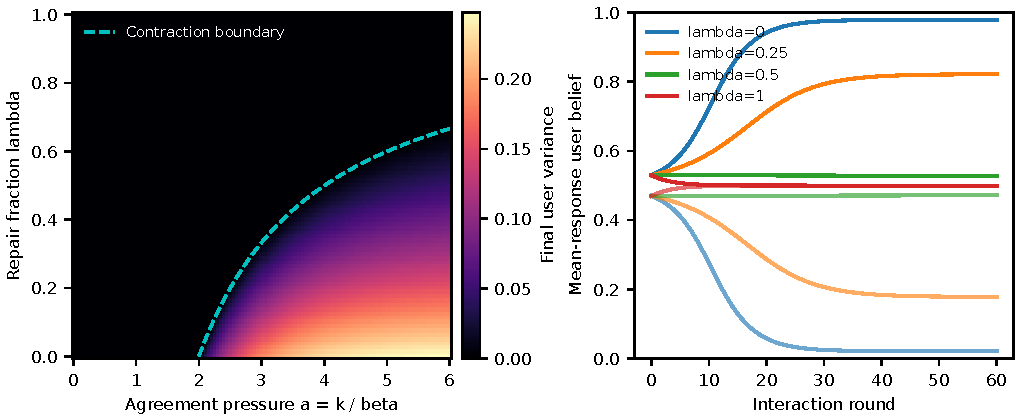
\includegraphics[width=.96\textwidth]{figures/phase.pdf}
\caption{Deterministic mean-response dynamics. Left: final
population variance after 400 updates from $s_0\in\{0.47,0.53\}$, $\eta=0.25$.
The dashed line is the strict-contraction boundary. Finite-horizon variance
remains nonzero near the boundary. Right: paired trajectories at $a=4$.
The simulations use the specified belief-update rule.}
\label{fig:phase}
\end{figure*}

\section{Stability guarantees and audit requirements}
Let $K_{x,s}$ be the preference policy's distribution over report values $q_c$. In kernel formulas, $\tau_x$ denotes its report pushforward $\sum_c\tau_x(c)\delta_{q_c}$, not a distribution on response text.
Assume a finite $L_x$ satisfies
$W_1(K_{x,u},K_{x,v})\le L_x|u-v|$, where $W_1$ is Wasserstein distance on
$[0,1]$. The same $\lambda_x$ must be used across non-evidential stances.
A stance-dependent repair fraction would introduce an additional feedback
term and requires a separate analysis.

\begin{theorem}[Stability budget and approximate full repair]
\label{thm:stability}
Fix $0<\eta\le1$. For the sampled update $U'=(1-\eta)U+\eta Q$,
the Markov kernel induced by
$K^\lambda_{x,s}=(1-\lambda_x)K_{x,s}+\lambda_x\tau_x$ is $W_1$-Lipschitz
with coefficient at most
\begin{equation}
 \rho_x=1-\eta+\eta(1-\lambda_x)L_x.
 \label{eq:rho}
\end{equation}
For a common evidence sequence with $\sup_x\rho_x<1$, differences between
initial belief distributions contract geometrically in $W_1$. This compares
belief laws, not the variance of independently sampled individuals.

Under full repair, suppose the implemented target $\widehat\tau_{x,s}$ differs
from a stance-independent ideal target by at most $\epsilon_t$ in total
variation at round $t$, uniformly over current belief states. Starting with the same initial belief and common
evidence, its belief law and the ideal target-driven law can be coupled so that
\begin{equation}
 \E|U_T-\widetilde U_T|
 \le\eta\sum_{t=0}^{T-1}(1-\eta)^{T-1-t}\epsilon_t.
 \label{eq:error}
\end{equation}
With a constant error bound, this is at most
$\epsilon[1-(1-\eta)^T]$.
\end{theorem}

If $L_x$ is known, a desired margin $\gamma\in(0,1)$ is obtained by choosing
$\lambda_x\ge\max\{0,1-(1-\gamma)/L_x\}$ for $L_x>0$, giving
$\rho_x\le1-\eta\gamma$. By convexity, $\KL(b_\lambda\|m_P)$ is
nondecreasing along $\lambda\in[0,1]$. Consequently, the smallest admissible
fraction minimizes the exact cost \emph{along this mixture path}; no
optimality over all stable policies is asserted. A positive margin avoids
the excluded boundary of a strict-contraction condition.

\begin{corollary}[A finite-audit expectation bound]
\label{cor:audit}
For $n\ge1$ independent class samples from a trusted target $\tau$ over $C$ classes,
the empirical frequency $\bar\tau$ satisfies
$\E\TV(\bar\tau,\tau)\le\tfrac12\sqrt{(C-1)/n}$.
For the add-$\alpha$ estimator
$\widehat\tau=(n\bar\tau+\alpha\boldsymbol1)/(n+C\alpha)$ with $\alpha\ge0$,
an upper bound is
\begin{equation}
 \E\TV(\widehat\tau,\tau)
 \le\min\left\{1,\frac12\sqrt{\frac{C-1}{n}}+
                   \frac{C\alpha}{n+C\alpha}\right\}.
 \label{eq:auditsamples}
\end{equation}
This controls target estimation error in expectation, not auditor bias.
\end{corollary}

\paragraph{Stability and correctness are distinct.}
An incorrect but stance-independent target can make the system stable and
wrong. Also, if unmeasured wording changes the interpreted epistemic signal,
the report-class map is not sufficient and Theorem~\ref{thm:stability} does not
cover that mechanism. Auditor validity and the sufficiency of the class
map are therefore separate requirements.

\subsection{From finite response audits to a stability certificate}
Equation~\eqref{eq:rho} requires a global sensitivity bound $L_x$.
Finite stance tests alone cannot establish it, even if the response
probability at every tested stance is known exactly.

\begin{proposition}[Finite stance audits need regularity]
\label{prop:finiteaudit}
For any finite set of audited stances $A\subset[0,1]$, there is a smooth,
bounded binary response probability $m(s)$ with $m(s)=1/2$ at every $s\in A$,
yet with two stable off-grid fixed points for
$F(s)=(1-\eta)s+\eta m(s)$, for every $0<\eta\le1$. Their separation can be
arbitrarily close to one. Thus, exact agreement with an invariant target on
finitely many stances cannot by itself certify global feedback stability.

Conversely, let $m\in C^2([0,1])$ satisfy a known global
curvature bound $|m''(s)|\le H$. Audit a uniform grid $s_j=(j-1)/(J-1)$ of $J\ge2$ points, spacing
$h=1/(J-1)$, with $n$ independent binary responses per point. Let
$\widehat m_j$ be the empirical means and
$\epsilon=\sqrt{\log(2J/\delta)/(2n)}$ for $0<\delta<1$.
With probability at least $1-\delta$,
\begin{equation}
 \sup_s|m'(s)|\le\widehat L_H:=
 \max_j\frac{|\widehat m_{j+1}-\widehat m_j|}{h}
       +\frac{2\epsilon}{h}+Hh/2.
 \label{eq:gridcertificate}
\end{equation}
This can be inserted into Equation~\eqref{eq:rho} for binary reports, where
the kernel $W_1$ distance equals the difference of response probabilities.
\end{proposition}

The $2\epsilon/h$ term penalizes overly fine grids at fixed observations per
point; $Hh/2$ penalizes overly coarse grids. For total report budget $N\simeq Jn$,
balancing the two errors gives $h$ of order $N^{-1/5}$ up to logarithms when
$H>0$ is fixed. A trustworthy curvature bound is additional information:
estimating it from the same unconstrained finite grid does not evade the first
part of the proposition. The certificate consequently trades sampling precision against coverage
under a supplied regularity assumption. It is pointwise in evidence context $x$; simultaneous certification of $M$ prespecified contexts requires, for example, a union bound using $\delta/M$. It does not certify an unrestricted set of unseen contexts.

\section{Report quality and belief dispersion}
Report Brier regret, conditional target TV, and excess simulated dispersion
measure different objects. With $Z\mid x\sim\mathrm{Bernoulli}(p_x)$
independent of report sampling conditional on evidence, define
\begin{equation}
 \mathcal R(\pi)=\E_{x,s,Y\sim\pi}(q_{c_x(Y)}-p_x)^2.
 \label{eq:ecr}
\end{equation}
Expected Brier loss equals this regret plus $\E_xp_x(1-p_x)$.
Target mismatch is $\E_{x,s}\TV(m_\pi,\tau_x)$; pooling first can erase
stance dependence. For a target-only baseline $\widetilde\pi$ with the
same initial population, evidence and sampling convention, define
\begin{equation}
 \mathrm{BPD}_T=\E_x[\Var(U_T^\pi\mid x)-\Var(U_T^{\widetilde\pi}\mid x)].
 \label{eq:bpd}
\end{equation}
This is signed excess dispersion, not a validated cognitive metric.
It can be zero under a common wrong consensus, so user mean-squared
evidence error is also required. Sampling variance in the target-only
baseline is not zero. Legacy CSV fields PCD and ECR are differences
in target TV and Brier regret from the reference, respectively.

\section{Experiments}
\subsection{Finite-action preference learning}
There are 21 forecast classes $q\in\{0,0.05,\ldots,1\}$ and three abstract
styles $z\in\{-1,0,1\}$, giving 63 responses. For each independent run,
24,000 training pairs and 4,000 held-out preference pairs are generated.
Each training context samples $p=0.05+0.9B$, $B\sim\operatorname{Beta}(0.8,0.8)$,
and $s\sim\operatorname{Uniform}(0.05,0.95)$. The reference has
\begin{equation}
 \begin{aligned}\pi_0(q,z\mid p)&\propto\nu(z)\exp[-(q-p_{\rm ref})^2/0.06],\\
 p_{\rm ref}&=0.5+0.65(p-0.5),\\ \nu&=(0.25,0.5,0.25).\end{aligned}
\end{equation}
The reward is
\begin{equation}
 \begin{aligned}r={}&-(q-p)^2-k(q-s)^2\\ &+0.8(2s-1)z+0.25(2q-1)(2s-1)z.\end{aligned}
 \label{eq:rewardexperiment}
\end{equation}
with $k=4$ and $\beta=0.5$ in the main setting. Pair labels follow
Bradley--Terry probabilities $\sig(r(y_a)-r(y_b))$. Candidate proposals are a
50:50 mixture of reference and uniform response sampling. The six supplied features contain the simulator reward exactly, up to a context-only constant: the ideal coefficient vector is $(0,-(1+k),2,2k,0.8,0.25)/\beta$. This is a well-specified low-dimensional learning test with direct access to $p$, not a test of learning evidence from text. We fit the DPO
pairwise likelihood using L-BFGS-B in the log-linear policy
$\pi_\theta\propto\pi_0\exp(\theta^\top\phi)$ with
$\phi=(q,q^2,qp,qs,z(2s-1),z(2s-1)(2q-1))$.
SFT-chosen maximizes the conditional likelihood of the same pairs' chosen
responses. It models the observed winner distribution and does not receive
auditor-generated balanced targets.

Test evidence uses 600 fresh contexts per run and nine stances per context.
Ten seeds yield 54,000 context--stance evaluations. The auditor target uses
Equation~\eqref{eq:target} with $T_E=0.01$. Audit-only uses this same target and
the reference style prior; CAEA uses the learned DPO class-conditionals.
Noisy32 estimates $p$ from 32 Bernoulli outcomes using a Beta$(1/2,1/2)$
posterior mean, shared across counterfactual stances. Audit-only-noisy32 uses the identical noisy target and reference style prior, equalizing target information with CAEA-noisy32. Oracle-nearest uses the known $p$ to select a closest grid report and retains the DPO conditional; it optimizes report risk rather than the prescribed spread target. Pooled-marginal repair geometrically averages the DPO class marginals over the nine stances and
retains DPO within-class distributions. Uniform-coverage sets all forecast
classes equally likely. Soft-score baselines reweight DPO by
$\exp[-v(q-p)^2/\beta]$ for $v\in\{0.5,2,8\}$; all settings are reported,
with no post-test selection of a winner.

For fitted DPO policies, reported KL is policy displacement. The exact
objective-cost identity applies to the fitted policy's implicit reward;
it need not equal a gap under the simulator's true reward after finite-data
estimation error.

\begin{table*}[t]
\centering\small
\caption{Finite-action results: means $\pm$ 95\% Student-$t$ confidence
half-widths over ten independent runs. Style is only the style component of
Equation~\eqref{eq:rewardexperiment}, not measured human helpfulness. Target
information is given to audit-based methods. KL is relative to learned DPO.}
\label{tab:main}
\begin{tabular}{lrrrr}\toprule
Method & Proper-score regret $\downarrow$ & Style reward $\uparrow$ & Target TV $\downarrow$ & KL to DPO\\\midrule
Reference & 0.0388 $\pm$ 0.0001 & 0.0000 $\pm$ 0.0000 & 0.4731 $\pm$ 0.0008 & 0.4825 $\pm$ 0.0126 \\
DPO & 0.0471 $\pm$ 0.0004 & 0.1946 $\pm$ 0.0058 & 0.5456 $\pm$ 0.0020 & 0.0000 $\pm$ 0.0000 \\
SFT-chosen & 0.0906 $\pm$ 0.0007 & 0.0502 $\pm$ 0.0032 & 0.6079 $\pm$ 0.0012 & 0.6095 $\pm$ 0.0101 \\
Audit-only & 0.0047 $\pm$ 0.0000 & 0.0000 $\pm$ 0.0000 & 0.0000 $\pm$ 0.0000 & 1.2537 $\pm$ 0.0153 \\
CAEA-0.5 & 0.0259 $\pm$ 0.0002 & 0.1943 $\pm$ 0.0062 & 0.2728 $\pm$ 0.0010 & 0.2798 $\pm$ 0.0035 \\
CAEA-1 & 0.0047 $\pm$ 0.0000 & 0.1940 $\pm$ 0.0066 & 0.0000 $\pm$ 0.0000 & 1.0480 $\pm$ 0.0101 \\
CAEA-noisy32 & 0.0096 $\pm$ 0.0002 & 0.1941 $\pm$ 0.0069 & 0.2826 $\pm$ 0.0059 & 1.1177 $\pm$ 0.0133 \\
Audit-only-noisy32 & 0.0096 $\pm$ 0.0002 & 0.0000 $\pm$ 0.0000 & 0.2826 $\pm$ 0.0059 & 1.3236 $\pm$ 0.0126 \\
Oracle-nearest & 0.0002 $\pm$ 0.0000 & 0.1940 $\pm$ 0.0067 & 0.7186 $\pm$ 0.0004 & 2.6851 $\pm$ 0.0107 \\
Pooled-marginal & 0.0397 $\pm$ 0.0003 & 0.1937 $\pm$ 0.0059 & 0.5224 $\pm$ 0.0029 & 0.1975 $\pm$ 0.0025 \\
Uniform-coverage & 0.1691 $\pm$ 0.0010 & 0.1954 $\pm$ 0.0052 & 0.6990 $\pm$ 0.0006 & 1.9819 $\pm$ 0.0119 \\
Soft-score-0.5 & 0.0444 $\pm$ 0.0003 & 0.1946 $\pm$ 0.0059 & 0.5354 $\pm$ 0.0020 & 0.0013 $\pm$ 0.0000 \\
Soft-score-2 & 0.0377 $\pm$ 0.0003 & 0.1944 $\pm$ 0.0059 & 0.5067 $\pm$ 0.0020 & 0.0176 $\pm$ 0.0002 \\
Soft-score-8 & 0.0227 $\pm$ 0.0001 & 0.1941 $\pm$ 0.0061 & 0.4125 $\pm$ 0.0021 & 0.1541 $\pm$ 0.0014 \\
\bottomrule\end{tabular}

\end{table*}

\paragraph{Predictive risk and conditional preferences.}
Table~\ref{tab:main} shows full repair decreasing report regret from 0.04707 to
0.00474, while the audit-only comparator has exactly the same regret. The shared audited marginal makes this equality necessary. The
comparison therefore isolates conditional preference retention rather
than independent recovery of the evidence target. CAEA retains positive style reward and costs less
KL than replacing the within-class distribution with the reference style
prior (1.04799 versus 1.25375). Half repair
gives intermediate report regret 0.02591 and KL 0.27976, with its regret and TV exactly determined by Equations~\eqref{eq:riskidentity}--\eqref{eq:tvidentity}. Noisy32 increases regret to 0.00962, exactly the same as Audit-only-noisy32. Oracle-nearest obtains regret 0.000206 at KL 2.68510, below the spread target's 0.00474 but with target TV 0.71858. This confirms that exact target matching is not Brier-risk optimality. Because the noisy target is shared over stances, its estimation error does not itself break full-repair stance invariance or the $1-\eta$ contraction; it changes the target-driven belief law and accuracy. Uniform forecast coverage has regret 0.16905:
more spread is not inherently epistemically better. Soft-score-8 has lower KL
than half repair and lower regret, but it does not match the audited marginal.
Matching a specified marginal and minimizing forecast risk under a KL
budget are different objectives; the repair does not dominate the latter.



\begin{table*}[t]
\centering\small
\caption{Exploratory paired uncertainty over contexts and label seeds.
Report difference is Head-DPO minus LM-base (negative is better);
style difference is CAEA-1 minus Audit-only (positive is better).
Intervals are percentile bootstrap intervals, not the seed-only
Student-$t$ half-widths in the supplementary seed-only table.}
\label{tab:paired}
\begin{tabular}{llrr}
\toprule
Backbone & Bank & $\Delta$ report regret [95\% CI] & $\Delta$ style match [95\% CI] \\
\midrule
SmolLM2-135M & original & -0.0164 [-0.0361, +0.0018] & +0.1406 [+0.0877, +0.1967] \\
SmolLM2-135M & permuted & +0.0168 [-0.0295, +0.0728] & -0.0469 [-0.1191, +0.0248] \\
Qwen2.5-0.5B & original & -0.0346 [-0.0530, -0.0171] & +0.1643 [+0.0961, +0.2353] \\
Qwen2.5-0.5B & permuted & +0.0047 [-0.0424, +0.0526] & -0.0084 [-0.0910, +0.0664] \\
\bottomrule
\end{tabular}

\end{table*}
\subsection{Pressure controls and stochastic feedback}
An additional 20 fitted DPO models use $k\in\{0,1,4,8\}$, five seeds each and
16,000 training pairs per fit. The learned reward coefficients are rescaled to
$\beta\in\{0.25,0.5,2\}$, which exactly changes DPO policy temperature in this
log-linear family without changing the fitted pairwise likelihood. Each is
evaluated on 1,000 fresh contexts with aligned ($s=p$), opposed ($s=1-p$), or
random stances. At $k=4,\beta=0.5$, average DPO regret is 0.02214 when aligned,
versus reference 0.03900; when opposed it is 0.07087. Thus, increased
preference agreement is not universally harmful.

Figure~\ref{fig:phase} evaluates the binary model in
Theorem~\ref{thm:blindness}.
At $a=4$, zero repair yields final mean-response variance 0.22920; full repair
reduces it to numerical zero. The $\lambda=0.5$ boundary is not assigned a
strict contraction guarantee. To distinguish mean-response behavior from sampling noise, we also simulate 5,000 independent user trajectories over
400 rounds, ten seeds, $\eta\in\{0.05,0.25\}$, and five repair fractions.
Full repair has stationary variance $\eta/[4(2-\eta)]$, not zero. At
$\eta=0.25$, measured full-repair variance is 0.03540 versus theoretical
0.03571, and unrepaired variance is 0.22959. Stochastic noise smooths the
deterministic phase picture; the mean-response boundary is not presented as a
zero-variance transition in the sampled process.

\subsection{Auditor uncertainty and semantic failure}
For 21 classes, an independent class-audit experiment samples the trusted
target at $p=0.73$, with $n\in\{8,16,32,64,128,256,512,1024\}$, 2,000
replicates each, and add-0.1 smoothing. Mean target TV is 0.17640 at $n=32$
and 0.03042 at $n=1024$, below the conservative expectation bounds 0.45687
and 0.07192. These are samples from a stipulated trustworthy class target;
they do not estimate bias in an LLM judge.

Two controls examine structural audit failure. When the true evidence probability is
0.8 but the full-repair auditor centers on 0.2, consensus remains stable and
converges near the wrong value. In a separate user mechanism where the literal
report stays at 0.5 but personalized wording adds an interpreted directional
cue $\delta\operatorname{sign}(s-0.5)$, limiting user variance is
$\delta^2$ despite zero literal-report regret. The class map misses a causally
relevant signal, so the report-only guarantee is inapplicable.

\paragraph{Response-audit certificate experiment.}
Separately from estimating the target, we sample the binary response kernel
$m(s)=\sig(4(2s-1))$, whose known curvature bound is
$H=2(4)^2/(3\sqrt3)$. For each total response budget
$N\in\{1024,4096,16384,65536,262144\}$, the grid size is planned from
$J\in\{5,9,17,33,65\}$ by minimizing $2\epsilon/h+Hh/2$ before observing
the audit samples. Five hundred independent binomial audit replicates per
budget are retained. With $\delta=0.05$ and contraction margin $\gamma=0.1$,
every realized certificate exceeds the true $L=2$ in these runs. The mean
sufficient repair fraction changes from 0.72965 to 0.62763 at the endpoints of the budget
range, versus 0.55 when $L$ is known exactly. The mean is not monotone at every intermediate budget because discrete grid changes also change the observed maximum secant slope; minimizing the remainder alone need not minimize the full realized certificate. A separate smooth bump
construction passes all nine grid-point audits exactly while having stable
off-grid beliefs at 0.13 and 0.87, with variance 0.1369.

\begin{figure*}[t]
\centering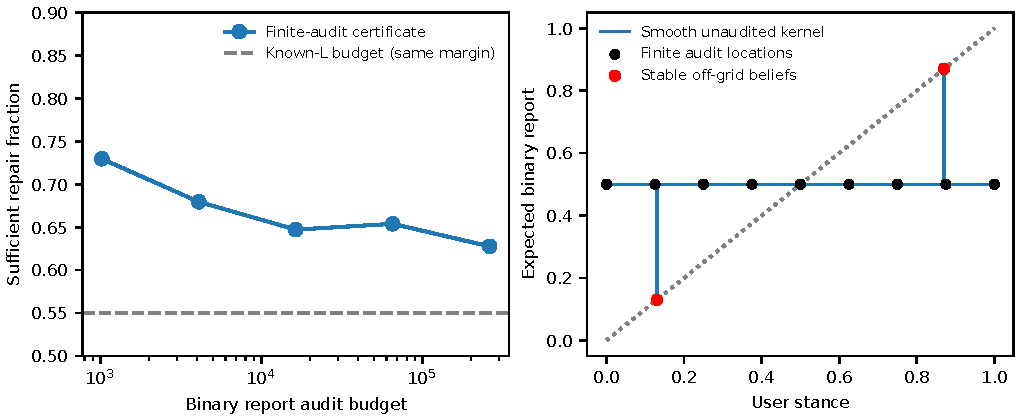
\includegraphics[width=.94\textwidth]{figures/audit_stability.pdf}
\caption{Response-audit budget and an explicit regularity failure. Left:
sufficient repair fractions from the curvature-dependent finite-sample
certificate, averaged over 500 audit replicates; the known-$L$ line uses the
same contraction margin. Right: narrow smooth off-grid deviations are exactly
invisible at all displayed audit locations. The supplied curvature assumption
is what rules out this failure in the certificate experiment.}
\end{figure*}



\subsection{Frozen-backbone candidate selection}
\label{sec:neural}
We evaluate a constrained candidate-selection interface on
SmolLM2-135M-Instruct and Qwen2.5-0.5B-Instruct \citep{smollm2,qwen25}.
Each prompt specifies a prior and signal likelihoods, allowing an analytic
Bayesian posterior. The evidence contexts are disjoint across training
(40), validation (12), and test (24) splits. Two unsupported user stances
per context yield 152 prompts per backbone, including 48 test prompts.
Ten one-token options encode five forecast values and two abstract styles.
Scores are normalized over these option letters; their mean unrestricted
next-token probability mass on the test split is 0.77433 for SmolLM2 and
0.91253 for Qwen.

All Transformer and original output-head weights remain frozen. A linear
ten-option decision-head adapter uses an intercept and 16 principal
components of final hidden states, fitted on training prompts only. We
optimize the DPO pairwise likelihood with 16 Bradley--Terry pairs per
training prompt and five label-sampling seeds. The regularization strength
is selected from $\{0.001,0.01,0.1\}$ using validation pair NLL. The reward
combines forecast error, agreement pressure $k=4$, and a 0.5 reward for the
requested abstract style. The evidence target uses $T_E=0.03$.



\paragraph{Conditional and unconditional retention.}
The fixed-bank results show that head-DPO lowers report regret relative
to both frozen bases. Full repair and Audit-only again have the same
regret, 0.01448, because they use the same class marginal. Full repair's
unconditional style-match rate is lower than head-DPO's, despite exact
preservation within each forecast class: changing the class mixture also
changes the aggregate style mixture. Conditional preservation therefore
does not guarantee unchanged overall style performance.

\paragraph{Answer-order sensitivity.}
An additional held-out control permutes the option-to-letter mapping
without retraining or model selection. On these prompts, report regret
is 0.20364 for the SmolLM2 base and 0.22048 for head-DPO; the corresponding
Qwen values are 0.21639 and 0.22107. Thus the initial head-DPO improvements
do not survive this control. Full-repair style-match rates fall to 0.45308
and 0.49155, below Audit-only's 0.5. The retained within-class policy can
itself encode position shortcuts. This pilot establishes execution on
frozen neural scores, while its transfer failures limit interpretation
of the learned selector.
With a correct, permutation-consistent class map and sufficient candidate
support, full repair enforces the specified class marginal even when the
input scores change. It does not remove position shortcuts within a class,
validate the class map, or guarantee unchanged aggregate style performance.


\paragraph{Paired evidence-context uncertainty.}
To avoid treating two stances from one evidence context as independent,
we replay the archived hidden states and fitted heads, average paired
differences within each of 24 test contexts, and independently resample
the five label seeds and 24 context clusters (5,000 crossed bootstrap
replicates). Table~\ref{tab:paired} reports exploratory percentile intervals,
conditional on the fixed training/validation split, backbone, and finite
evidence grid. These do not cover training-context variation. For SmolLM2,
the original-bank report-regret difference already has an interval spanning
zero; for Qwen it is negative on the original bank. Both permutation-control
intervals span zero. Full repair's positive style advantage on the original
bank is not established after permutation. These results narrow the evidence
for transfer rather than repairing the failed selector. This revision
replays archived inference and does not claim a fresh model run. Maximum
absolute deviation from recorded summary values is $5.91\times10^{-8}$,
consistent with replay roundoff in the archived float32 PCA features.





\section{Discussion and limitations}
Three distinctions govern interpretation. First, stability does not imply
correctness: a stance-independent incorrect target can stabilize a false
consensus. Our oracle or sampled targets isolate repair and do not solve
evidence assessment. Increasing samples does not remove systematic auditor
bias. Second, report classes must capture the signal driving the specified
update; unmeasured persuasive wording invalidates that representation.
Third, the deterministic bifurcation is not a zero-variance transition or
a nonergodicity claim for the sampled process.

The main learner has six supplied features containing the true synthetic
reward. The neural pilot uses frozen features, ten supplied options,
24 test evidence contexts and five label seeds. Its answer-order failures
remain negative results. Neither the finite-grid theorem nor these pilots
certify an unrestricted language model: the global regularity and
evidence-context coverage assumptions have not been established for it.

The next empirical test needs an independently evaluated non-oracle audit,
equal evidence/candidate access across methods, unseen responses, and
separate tests of unsupported pressure and informative new evidence.
Free-text helpfulness and human belief effects require direct measurement;
larger models alone do not establish them. Prospective human studies would
also require applicable ethical review. The released controlled results
support the stated observability and conditional-repair distinctions.

\section{Conclusion}
Pooled one-turn output quality does not identify feedback stability in the
constructed preference-based interaction. CAEA makes the intervention
explicit: repair an audited epistemic marginal, retain the preference
policy within each class, and quantify the resulting objective cost.
Contraction bounds connect repair strength to feedback control, while
finite-audit results show why certification requires additional regularity.
The controlled experiments support these distinctions and expose their
dependence on auditor validity, response representation, and the update
model. Together, the results provide a framework for separating what a
preference policy says in isolation from how its conditional behavior can
shape repeated belief updates.

\section*{Broader impact statement}
The analysis can help distinguish output accuracy from feedback stability,
but it does not justify deploying a system to steer users toward an
unverified belief target. An incorrect auditor can stabilize false beliefs;
a narrow class map can omit persuasive cues, and mandatory target matching
can suppress warranted disagreement or minority perspectives. An application
would need independent evidence assessment, explicit uncertainty and
abstention, scrutiny of target selection, and evaluation of users' actual
interpretations. We do not offer a validated safeguard against these risks.
The experiments use generated data and public pretrained models, without
human participants or collected personal conversations.


\clearpage
\bibliographystyle{named}
\bibliography{references}
\end{document}
